\makeatletter
\def\input@path{{../styles/}{../../styles/}{../../../styles/}{../}{../../}{../../../}}
\makeatother
\documentclass{ee102_notes}
% macros.tex - Course meta information
\renewcommand{\course}{EE 102}
\renewcommand{\coursetitle}{Signal Processing and Linear Systems}
\renewcommand{\instructor}{Ayush Pandey}
\renewcommand{\semester}{Fall}
\renewcommand{\year}{2025}
\renewcommand{\shorttitle}{Week 1: Introduction to Signals}
% Use \renewcommand to avoid 'already defined' errors

% The following packages can be found on http:\\www.ctan.org
% \usepackage{graphics} % for pdf, bitmapped graphics files
%\usepackage{epsfig} % for postscript graphics files
%\usepackage{mathptmx} % assumes new font selection scheme installed
%\usepackage{times} % assumes new font selection scheme installed
\usepackage{amsmath} % assumes amsmath package installed
\usepackage{amssymb,mathtools}  % assumes amsmath package installed
\usepackage{xcolor}
\usepackage{pgfplots,subcaption}
\usepackage[hidelinks]{hyperref}
\usepackage{verbatim}
\usepackage{graphicx}
\usepackage{listings}
\usepackage{fancyhdr}
% \usepackage{geometry}
\usepackage{siunitx}
\usepackage[most]{tcolorbox}
\usepackage{enumitem}
\usepackage{environ}
% -------- listings (Python) ----------
\lstdefinestyle{py}{
  language=Python,
  basicstyle=\ttfamily\small,
  keywordstyle=\color{blue!60!black}\bfseries,
  commentstyle=\color{green!40!black},
  stringstyle=\color{orange!60!black},
  showstringspaces=false,
  columns=fullflexible,
  frame=single,
  framerule=0.3pt,
  numbers=left,
  numberstyle=\tiny,
  xleftmargin=1em,
  tabsize=2,
  breaklines=true,
}

\usepackage[american]{circuitikz}
\usepackage{tikz}
\usetikzlibrary{arrows.meta,positioning,calc,angles,quotes}
\tikzset{
  >={Latex[length=2.2mm]},
  block/.style={draw, thick, rectangle, minimum height=10mm, minimum width=24mm, align=center},
  gain/.style={block, minimum width=14mm},
  sum/.style={draw, thick, circle, inner sep=0pt, minimum size=6mm},
  conn/.style={-Latex, thick},
}
\usepackage{caption}    
\usepackage{lscape}
\usepackage{soul}
\usepackage{physics}
\usepackage{hyperref}
\hypersetup{
    colorlinks=true,
    linkcolor=blue,
    filecolor=magenta,      
    urlcolor=blue,
    pdftitle={week1_notes},
    pdfpagemode=FullScreen,
}
%\usepackage{float} 

%\usepackage[demo]{graphicx}
\pgfplotsset{compat=1.18}
% \usepgfplotslibrary{fillbetween}

\newsavebox{\measurebox}

\let\proof\relax\let\endproof\relax


\def\abs#1{\left\lvert#1\right\rvert}
\let\proof\relax
\let\endproof\relax
\usepackage{amsthm}
\usepackage{accents}
\usepackage{relsize}
\newcommand{\ubar}[1]{\underaccent{\bar}{#1}}
\newtheorem{theorem}{Theorem}
\newtheorem{corollary}{Corollary}[theorem]
\newtheorem{lemma}{Lemma}
\newtheorem{proposition}{Proposition}
\newtheorem{statement}{Statement}

\theoremstyle{definition}
\newtheorem{definition}{Definition}
 
\theoremstyle{remark}
\newtheorem*{remark}{Remark}
\theoremstyle{remark}
\newtheorem*{claim}{Claim}
\setlength{\parindent}{0cm}
\newenvironment{nalign}{
    \begin{equation}
    \begin{aligned}
}{
    \end{aligned}
    \end{equation}
    \ignorespacesafterend
}

\renewcommand{\releasedate}{September 29, 2025}

\newcommand{\Eblank}{\rule{3cm}{0.4pt}}
\newcommand{\Rankblank}{\rule{3cm}{0.4pt}}

\begin{document}

\section*{EE 102 Week 5, Lecture 1 (Fall 2025)}
\subsection*{Instructor: \instructor}
\subsection*{Date: \releasedate}

\section{Goals}

\section{Review: LTI systems and convolutions}
Recall that using the linearity and time-invariance of the system, we can define the output, $y(t)$ of the system to any arbitrary input $x(t)$ in terms of the impulse response of the system $h(t)$ using the following integral:
\begin{equation}
y(t) = (x * h)(t) = \int_{-\infty}^{\infty} x(\tau) h(t - \tau) d\tau.
\label{eq:convolution}
\end{equation}
This integral is called the convolution integral. 
\begin{popquiz}
Using the convolution integral, show that you recover the impulse response $h(t)$ when the input is $\delta(t)$. As a consequence, you will have proven that the convolution of a signal (in this case, $h(t)$) with an impulse is equal to the same signal. 
\popqsplit
Substitute $x(t) = \delta(t)$ in equation~\eqref{eq:convolution} to write
\[
y(t) = (x * h)(t) = \int_{-\infty}^{\infty} \delta(\tau) h(t - \tau) d\tau.
\]
Since $\delta(\tau)$ is non-zero only when $\tau = 0$, we have 
\[
y(t) = h(t)\int_{-\infty}^{\infty} \delta(\tau) d\tau
\]
with $h(t)$ out of the integral since it does not depend on $\tau$ (the integration variable). Notice that the integral is equal to 1 (definition of the impulse signal). So, we get the desired result $y(t) = h(t)$. Additionally, notice that $\delta(t) * x(t) = x(t)$ --- holds true in general for any signal.
\end{popquiz}

\section{Time-domain system response}
In this section, we discuss the response of systems in time-domain. We focus our discussion on linear systems and their responses. The \ul{overarching message about linear systems} is the following: if you \emph{know} how the system responds under a given condition or an input, then you can construct the system output if any linear combination of the known conditions occur. In other words, you can use the isolated system response to obtain the output to a new input that is a linear combination of the inputs for which you have the data already. This is called the \emph{principle of superposition} (note that the above is only an informal description). 

We often find it useful to talk about two kinds of system outputs: (1) the ``natural'' or the characterisitic output of the system when there are no forcing inputs, and (2) the output of the system to forced inputs. For linear systems, we can add these two outputs to get the full output of the system when both are present simultaneously.

\subsection{Building intuition for a system's responses}
Consider yourself --- a student invested in learning new things --- as a system. As you stroll past the lakes in and around the campus, you must have observed that the number of birds increases through late fall and winter and then thins from late spring into the hot, dry summer. Without anyone explicitly teaching you the ecology of bird movement, you self-learn and update your knowledge about bird movement as you observe these patterns and correlate them with the season. This is your natural response as a ``system'' that is invested in learning new things. Simultaneously, if you enroll in an ecology class as you expand your general education, you might be ``forced'' to learn (due to the pressure of exams!) that the Central Valley lies on the Pacific Flyway. Large flocks of geese, cranes, and ducks concentrate here from roughly October through February and by early summer many waterfowl have departed north to breeding grounds. This learning will be your response to the external input (the instruction in the ecology course). Your overall learning (if your learning progresses linearly) is the sum of your self-learned concepts and the concepts from the course. In this case, a nonlinear learner can have an advantage --- one who accentuates their overall learning by synthesizing new (extra) knowledge by combining the natural (self-learning) and forced learning in innovative ways.


We conclude by writing the output of any general linear system as a combination of the natural/characteristic/initial condition response and the forced response. For a system with initial condition $x_0$ and an input $u(t)$, we write the output $y(t)$ as
\[
y(t) = y_{0}(t) + y_{\text{forced}}(t)
\]
where $y_0(t)$ is the initial condition response to initial condition $x_0$. This is the characteristic response of the system without any forced inputs (the self-learning by seeing initial conditions, in the example above). Finally, $y_{\text{forced}}(t)$ is the forced response, that is, the output of the system when only the forced input $u(t)$ is present in isolation (the forced course-based learning, in the example above). 
\subsection{Example: Analyzing an RC circuit using convolution}
Consider a series RC circuit shown in the diagram~\ref{fig:rc-circuit}. Assume that we have an input voltage $u_{\text{in}}(t)$ that can be applied to the circuit using a function generator and the capacitor can have an initial voltage $v_0$ volts at time $t = 0$. We denote the output voltage for the circuit as the voltage across the capacitor $v_{\text{out}}(t)$. 
\begin{figure}
\centering
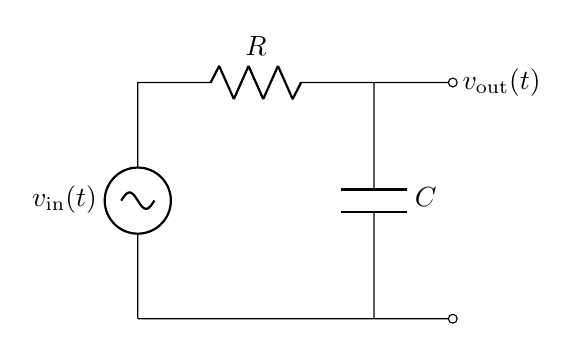
\begin{tikzpicture}
    \draw
    % don't connect v_in to ground. it is a voltage source
    (0,0) to[vsourcesin, l=$v_{\text{in}}(t)$] (0,3)
    to[R, l=$R$] (3,3)
    to[C, l=$C$] (3,0)
    to[short, ] (0,0)
    (3,3) to[short, -o] (4,3) node[right] {$v_{\text{out}}(t)$}
    (3,0) to[short, -o] (4,0) node[right] {};

\end{tikzpicture}
\caption{An RC circuit with input voltage $v_{\text{in}}(t)$ and output voltage $v_{\text{out}}(t)$.}
\label{fig:rc-circuit}
\end{figure}
A typical analysis of such circuits uses differential equations to describe and compute the system response (recall pre-requisite \#3 where you solved a differential equation to solve this circuit). Here, we will use convolution to find the output of the system to various common types of inputs: 

\begin{itemize}
\item an impulse input at $t=0$
\item a step input voltage (modeling DC input)
\item a sinusoidal voltage input (modeling AC input)
\item a generalized complex exponential input signal
\end{itemize}

\begin{popquiz}
    Before we jump into the application of convolution to the RC circuit example, it is important to ensure that the assumptions for the convolution integral to hold are still met. Your task is to state these assumptions (linearity and time-invariance) and prove that the RC circuit is linear and time-invariant. Additionally, also prove that the RC circuit is a causal system.
    \popqsplit
    Hints:
    
    For linearity, prove that the principle of superposition holds for the system. Assume that for inputs $u_1$ and $u_2$, the outputs are $y_1$ and $y_2$. 
    Then, write the system description using KVL (forward refer to the next pop quiz for a simple derivation of the following):
    \begin{equation}
        \label{eq:y1}
    \dot y_1(t)+\frac{1}{RC}\,y_1(t)=\frac{1}{RC}\,u_1(t),
    \end{equation}
    \begin{equation}
    \dot y_2(t)+\frac{1}{RC}\,y_2(t)=\frac{1}{RC}\,u_2(t),
    \label{eq:y2}
    \end{equation}
    Now, for an input $k_1u_1 + k_2u_2$, find the output $y^*$ and show that it is equal to $k_1y_1 + k_2y_2$ by using equations~\eqref{eq:y1} and~\eqref{eq:y2}. 

    For time-invariance, consider one of the input-output pairs, say equation~\eqref{eq:y1} and a time-shifted input $u_1(t - t_1)$. Prove that the output to the time-shifted input is the same as applying time-shift in the original output $y_1$.

    For causality, note that the voltage output is zero for all negative time in a RC circuit. Therefore, it is a causal system.
\end{popquiz}

\subsubsection{An impulse input to an RC circuit}
An impulse at $t = 0$ is simply given by $v_0\delta(t)$, where $v_0$ is the magnitude of the impulse (the area under the curve of this impulse is $v_0$). From the pop quiz at the beginning of this lecture, you know that the output of the system (with zero initial conditions) to an impulse is just the impulse response. Since the system is linear (see pop quiz above), the output of the system to a scaled impulse $v_0\delta(t)$ will be equal to   
\[
y(t) = v_0 h(t)
\] 
where $v_0$ is the magnitude of the input impulse (the area under curve). To find the impulse response of the RC circuit, we will have to rely on our circuits knowledge --- signal processing can only get us so far! From circuit theory, we know that an initial impulse on the circuit will cause a jump in the voltage and then an exponential decay (with a time constant of $RC$) through the resistor in the circuit. Full proof of this fact can be found in the solution of the pop-quiz below. We have the impulse response of an RC circuit (response to unit impulse)
\begin{equation}
\label{eq:h-rc}
h(t) = \frac{1}{RC}e^{-\frac{t}{RC}}u(t)
\end{equation}

Therefore, the output to the scaled impulse is $y(t) = \frac{v_0}{RC} e^{-\frac{t}{RC}}u(t)$.

\begin{popquiz}
Prove that the impulse response of an RC circuit is given by equation~\eqref{eq:h-rc}.
\popqsplit
Start by writing the KVL for the series RC circuit. The input is the applied source voltage $v_{\text{in}}(t)$ and the output is the capacitor voltage $v_{\text{out}}(t)$. KVL gives
\[
v_{\text{in}}(t)=v_R(t)+v_C(t)=R\,i(t)+v_{\text{out}}(t),
\]
where $i(t)$ is the series current and
\[
v_{\text{out}}(t)=\frac{1}{C}\int i(t)\,dt,
\]
with the constant of integration set by the initial capacitor voltage. Differentiating $v_{\text{out}}$ yields $i(t)=C\,\dot v_{\text{out}}(t)$. Substituting into KVL gives a first-order ODE in one variable:
\[
\dot v_{\text{out}}(t)+\frac{1}{RC}\,v_{\text{out}}(t)=\frac{1}{RC}\,v_{\text{in}}(t).
\]

The homogeneous (natural) solution for arbitrary initial condition $v_{\text{out}}(0^-)=v_0$ is
\[
v_{\text{out}}(t)=v_0\,e^{-t/(RC)}.
\]
This is the \emph{natural response} of the system due to the initial capacitor voltage.

To compute the \emph{impulse response}, drive the circuit with a unit impulse input and set zero initial voltage:
\[
v_{\text{in}}(t)=\delta(t),\qquad v_{\text{out}}(0^-)=0.
\]
Using the ODE above,
\[
\dot v_{\text{out}}(t)+\frac{1}{RC}\,v_{\text{out}}(t)=\frac{1}{RC}\,\delta(t).
\]
Using the integrating factor method, you can write 
\[
\frac{d}{dt}\!\left(e^{t/(RC)}\,v_{\text{out}}(t)\right)=\frac{1}{RC}\,e^{t/(RC)}\delta(t).
\]
Since the system is causal, $v_{\text{out}}(t)=0$ for $t<0$ and the initial voltage is zero, so $v_{\text{out}}(0^-)=0$. Integrating from $0^-$ to $t>0$ gives
\[
e^{t/(RC)}\,v_{\text{out}}(t)-0=\frac{1}{RC}\!\int_{0^-}^{t}\!e^{\tau/(RC)}\delta(\tau)\,d\tau
=\frac{1}{RC}.
\]
Hence, for $t > 0$, the impulse response is 
\[
h(t) = v_{\text{out}}(t)=\frac{1}{RC}\,e^{-t/(RC)}.
\]
For a general definition of the impulse response that holds for all time, we can include causality using the unit step $u(t)$ function as
\[
h(t)=\frac{1}{RC}\,e^{-t/(RC)}\,u(t).
\]
Note that the units of the impulse response are $1/\text{seconds}$ so that the convolution $(h*x)(t)$ has units of volts (the units of output signal --- $v_{\text{out}}(t)$).

\end{popquiz}

\subsubsection{A step input to an RC circuit}
Let's compute the forced input response of the RC circuit for a scaled step input that models a DC voltage applied to the circuit $x(t) = v_{\text{DC}} u(t)$. By applying the convolution integral, we can compute the system output $y(t)$ as 
\[
y(t) = \int_{-\infty}^{\infty} v_{\text{DC}} u(\tau) h(t - \tau) d\tau
\]
which can be evaluated as
\[
y(t) = v_{\text{DC}} \int_{0}^{t} h(t - \tau) d\tau
\]
since the step function is zero for $\tau < 0$ and $h(t - \tau)$ is zero for $\tau > t$ (causality of the real-life RC circuit's voltage response). To further understand this, you can see that the step input of the DC voltage is only applied at time $t = 0$. So, anything for negative time is 0. Similarly, you will see that the impulse response of the system will be zero for any negative time. Therefore, we can limit the integration limits to $0$ and $t$. Next, we can substitute the impulse response from equation~\eqref{eq:h-rc} to get
\[
y(t) = \frac{v_{\text{DC}}}{RC} \int_{0}^{t} e^{-\frac{t - \tau}{RC}} d\tau.
\]
Evaluating this integral, we get
\begin{equation}
    \label{eq:step-RC}
y(t) = \frac{v_{\text{DC}}}{RC} \left(1 - e^{-\frac{t}{RC}}\right)u(t).
\end{equation}
This is the forced response of the RC circuit to a step input voltage. 

\subsubsection{A sinusoidal input to an RC circuit}
We can compute the forced response of the RC circuit to a sinusoidal input voltage $x(t) = v_{\text{AC}} \cos(\omega t) u(t)$. Using the convolution integral, we can write
\[
y(t) = \int_{-\infty}^{\infty} x(\tau) h(t - \tau) d\tau.
\]
Substituting the expressions for $x(t)$ and $h(t)$, we get
\begin{equation}
    \label{eq:sine-RC}
y(t) = \int_{0}^{t} v_{\text{AC}} \cos(\omega \tau)\frac{1}{RC} e^{-\frac{t - \tau}{RC}} d\tau.
\end{equation}
Evaluating this integral will give us the forced response of the RC circuit to the sinusoidal input. This is same as the pre-requisite \#3 problem set! As you might remember, integrating the above requires a bit of effort as it is an integration by parts. Later on in this course, we will solve this using an easier method.
\subsubsection{A generalized complex exponential signal input to an RC circuit}
For a complex exponential signal, note that we are aiming for analysis of a broader variety of possible real signals. As we have seen before, complex exponentials can be used to define sinusoids, exponentials, and their combinations. By isolating the real and imaginary parts as needed, we can get a large class of signals as a subset of the general complex exponential signal $x(t) = A e^{st}$ where $A$ and $s$ are complex numbers. We can apply the convolution integral~\eqref{eq:convolution} to compute the output of the signal $y(t)$ to this input. As expected, the output will also be a complex signal and its special cases will lead to the computation of the output of the system for the input signal represented in that special case. 
For zero initial conditions, we write the convolution equation for this input as
\[
y(t)=\int_{0}^{t} A e^{s\tau}\,\frac{1}{RC}e^{-\frac{t-\tau}{RC}}\,d\tau
= \frac{A}{RC}\,e^{-t/(RC)} \int_{0}^{t} e^{\left(s+\frac{1}{RC}\right)\tau}\,d\tau.
\]
Evaluating the integral,
\[
y(t)= \frac{A}{RC}\,e^{-t/(RC)}\,\frac{e^{\left(s+\frac{1}{RC}\right)t}-1}{\,s+\frac{1}{RC}\,}
= A\,\frac{e^{s t}-e^{-t/(RC)}}{\,1+sRC\,}\,u(t).
\]
By further manipulating the above, we can see that it is made up of two parts:
\begin{equation}
    \label{eq:output-complex}
y(t) = Ae^{st}\,\frac{1}{\,1+sRC\,}\,u(t) - A\,\frac{e^{-t/(RC)}}{\,1+sRC\,}\,u(t).
\end{equation}
This is an interesting result due to many properties that we can observe from the output:
% comment on linearity and how input appears, comment on the transient part, and that it dies down, leaving the response to forced input, and then also comment on the special cases explicitly and get that the output comes out to be the same as the previous cases and same output as we have seen in other standard input cases.

\textbf{Observation 1:} The system is linear. We observe the output that the output has the same ``shape'' as the input. Because the system is linear, the complex exponential input $A e^{st}$ reappears in the output multiplied by a constant factor $\frac{1}{1+sRC}$. That first term,
  \[
  y_{\text{forced}}(t)=A\,\frac{e^{st}}{1+sRC}\,u(t),
  \]
  is the \emph{forced (particular) response}. This is what you would derive by integrating the differential equation by parts! Here, we did the same but in two lines of algebra and a very simple integration instead --- the power of exponentials!

\textbf{Observation 2:} The transient term decays to 0. The second term,
  \[
  y_{\text{transient}}(t)=-A\,\frac{e^{-t/(RC)}}{1+sRC}\,u(t),
  \]
  is the \emph{transient (natural) response}. It always decays like $e^{-t/(RC)}$, so for large $t$ the output approaches the forced response, the transient part will disappear to 0 as $t\to\infty$.

\textbf{Observation 3:} As promised, the complex exponential is useful because it specializes to many other simple cases we derived individually above.

\textbf{\ul{Special case 1:} Unit step.} Note that by setting $s=0$, $A=v_{\text{DC}}$, we get 
    \[
    y(t)=v_{\text{DC}}\big(1-e^{-t/(RC)}\big)u(t),
    \]
    which matches the step-response derived above in equation~\eqref{eq:step-RC}.

\textbf{\ul{Special case 2:} Real exponential.} Although we did not derive this earlier, we can now easily compute the output of the RC circuit to an exponential input $x(t) = Ae^{\alpha t}$. For this, set $s=\alpha\in\mathbb{R}$, and choose $A$ to be a real in the general form. Then, we have
    \[
    y(t)=A\,\frac{e^{\alpha t}-e^{-t/(RC)}}{1+\alpha RC}\,u(t).
    \]

\begin{popquiz} 
Remind yourself and derive the sine signal from the complex exponential: Prove that a real input signal $x(t)=A_{\text{AC}}\sin(\omega t)$ can be obtained from the general complex exponential $x_c(t)=A e^{st}$ by taking an appropriate real (or imaginary) part. In particular, show that $x(t)$ is the imaginary part of the general complex exponential for a suitable choice of $A$ and $s$. 
% \[
% x(t)=\Im\!\big\{A_{\text{AC}} e^{j\omega t}\big\}.
% \]
\popqsplit
For $s = j\omega$ and $A = A_{\text{AC}}$ and taking the imaginary part, we get
\[
\Im\!\big\{A_{\text{AC}}e^{j\omega t}\big\}
=\Im\!\big\{A_{\text{AC}}\cos(\omega t)+jA_{\text{AC}}\sin(\omega t)\big\}
=A_{\text{AC}}\sin(\omega t).
\]
where we used the Euler's identity $e^{j\omega t}=\cos(\omega t)+j\sin(\omega t)$ to expand the complex exponential. This is not the only way to obtain the sine function from the generalized complex exponential. An alternative is to set $s=j\omega$ and $A=-jA_{\text{AC}}$ and take the real part:
\begin{align*}
\Re\!\big\{(-jA_{\text{AC}})e^{j\omega t}\big\}
&=\Re\!\big\{-jA_{\text{AC}}\cos(\omega t)-j^2A_{\text{AC}}\sin(\omega t)\big\}\\
&=\Re\!\big\{-jA_{\text{AC}}\cos(\omega t)+A_{\text{AC}}\sin(\omega t)\big\}.
\end{align*}
The first term is purely imaginary, so its real part is $0$, and the second term is real. Hence
\[
\Re\!\big\{(-jA_{\text{AC}})e^{j\omega t}\big\}
= A_{\text{AC}}\sin(\omega t).
\]
\end{popquiz}


\textbf{\ul{Special case 3:} Sinusoidal input.} With $s=j\omega$, $A$ real (see pop quiz above), take the real part of
    \[
    y(t)=A\,\frac{e^{j\omega t}-e^{-t/(RC)}}{1+j\omega RC}\,u(t).
    \]
For large $t$, the transient dies out and the output is a sinusoid with scaled amplitude and a phase lag, consistent with the earlier sinusoidal case (see equation~\eqref{eq:sine-RC}). In fact, note that we did not derive the output in closed form earlier (due to fear of the ugly integration by parts!). Now we have the answer to the same input but obtained in a much easier way. 

\textbf{Observation 4:} If the input grows ($\Re\{s\}>0$), the forced term grows accordingly; the RC remains stable (its transient decays), but a growing input produces a growing output.
\begin{popquiz}
    Is the RC circuit bounded input bounded output stable? 
    \popqsplit 
    For any bounded input $x(t)$, we have $|x(t)| < M$ for some finite $M$ and all time $t$. The output is given by the convolution integral
    \[
    y(t) = \int_{-\infty}^{\infty} x(\tau) h(t - \tau) d\tau.
    \]
    Since $|x(\tau)| < M$, we can write
    \[
    |y(t)| \leq \int_{-\infty}^{\infty} |x(\tau)| |h(t - \tau)| d\tau < M \int_{-\infty}^{\infty} |h(t - \tau)| d\tau.
    \]
    Since the impulse response of the RC circuit is given by equation~\eqref{eq:h-rc}, we can evaluate the integral to get
    \[
    |y(t)| < M \int_{0}^{\infty} \frac{1}{RC} e^{-\frac{t - \tau}{RC}} d\tau = M.
    \]
    Therefore, the output is bounded by $M$ for all time $t$. Hence, the RC circuit is bounded input bounded output stable.

    An alternative way is to start from equation~\eqref{eq:output-complex} to show in a single step that $y(t)$ is bounded as long as the input $Ae^{st}$ is bounded. 
\end{popquiz}

\section{Next class}
In the next class, we will talk about an image processing example using convolution and will visualize convolution further. 
\end{document}
